\begin{frame}{Earth Observation Data Is Not ImageNet}
  \begin{itemize}\footnotesize\itemsep0.25em
    \item \textbf{Many bands:} Sentinel-2 samples 13 bands centred from 443 to about 2190\,nm, visible to short-wave infrared. Indices combine bands: NDVI, the normalised difference vegetation index, is $(\mathrm{NIR}-\mathrm{Red})/(\mathrm{NIR}+\mathrm{Red})$, with NIR the near-infrared band.
    \item \textbf{Ground sampling distance (GSD):} the ground distance between neighbouring pixel centres. At 10\,m GSD a car is smaller than one pixel.
    \item \textbf{Time and cloud:} every place is revisited every few days, but clouds hide optical dates, so each pixel is an irregular time series. Synthetic aperture radar (SAR) images through cloud, day and night.
  \end{itemize}
  \vspace{0.2em}
  {\centering\scriptsize
  \begin{tabular}{>{\raggedright\arraybackslash}p{1.9cm} >{\raggedright\arraybackslash}p{2.6cm} >{\raggedright\arraybackslash}p{3.7cm} >{\raggedright\arraybackslash}p{3.5cm}}
    \toprule
     & \textbf{Web photo (ImageNet)} & \textbf{Sentinel-2 (optical)} & \textbf{Sentinel-1 (radar)} \\
    \midrule
    Sensor & camera, 3 bands (RGB) & multispectral imager, 13 bands & C-band SAR \\
    Resolution & unknown, varies & 10, 20 or 60\,m GSD & 5\,m $\times$ 20\,m (main land mode) \\
    Revisit & one shot & 10 days per satellite, 5 with two & repeats every 12 days, 6 with two \\
    Light and weather & -- & daylight, clear sky & day and night, any weather \\
    Delivered as & JPEG, a few hundred pixels & 110\,km $\times$ 110\,km tiles: about 11{,}000 $\times$ 11{,}000 pixels per 10\,m band & 250\,km wide swath \\
    \bottomrule
  \end{tabular}\par}
  \vspace{0.2em}
  {\scriptsize Sources: ESA SentiWiki, \href{https://sentiwiki.copernicus.eu/web/s2-mission}{S2 mission}, \href{https://sentiwiki.copernicus.eu/web/s2-products}{S2 products} and \href{https://sentiwiki.copernicus.eu/web/s1-mission}{S1 mission} pages.\par}
\end{frame}

\begin{frame}{Foundation Models for Bands, Time, and Place}
  \begin{columns}[T,onlytextwidth]
    \column{0.52\textwidth}
      \begin{itemize}\footnotesize\itemsep0.2em
        \item \textbf{SatMAE} (NeurIPS 2022): MAE for satellites: a temporal embedding, patches masked independently across dates, and spectral position encodings per band group.
        \item \textbf{Prithvi-EO-2.0} (NASA and IBM, released 2024): patches from each date of a four-date series. Latitude, longitude, year and day of year enter as sin/cos codes with learned weights, dropped with probability 0.1 in pretraining so the model also runs without them. ViT-L (300M) and ViT-H (600M), pretrained on 4.2 million time series at 30\,m.
        \item \textbf{DOFA} (Dynamic One-For-All, 2024): one encoder for any sensor. A hypernetwork turns each band's central wavelength into its patch-embedding weights; pretrained on five sensors with 2 to 202 channels.
        \item \textbf{TerraMind} (ICCV 2025): any-to-any generation across nine modalities, among them radar, optical, elevation, land cover, NDVI and captions, learned by masked-token prediction on about 9 million aligned samples.
      \end{itemize}
    \column{0.46\textwidth}
      \centering
      \vspace{0.3em}
      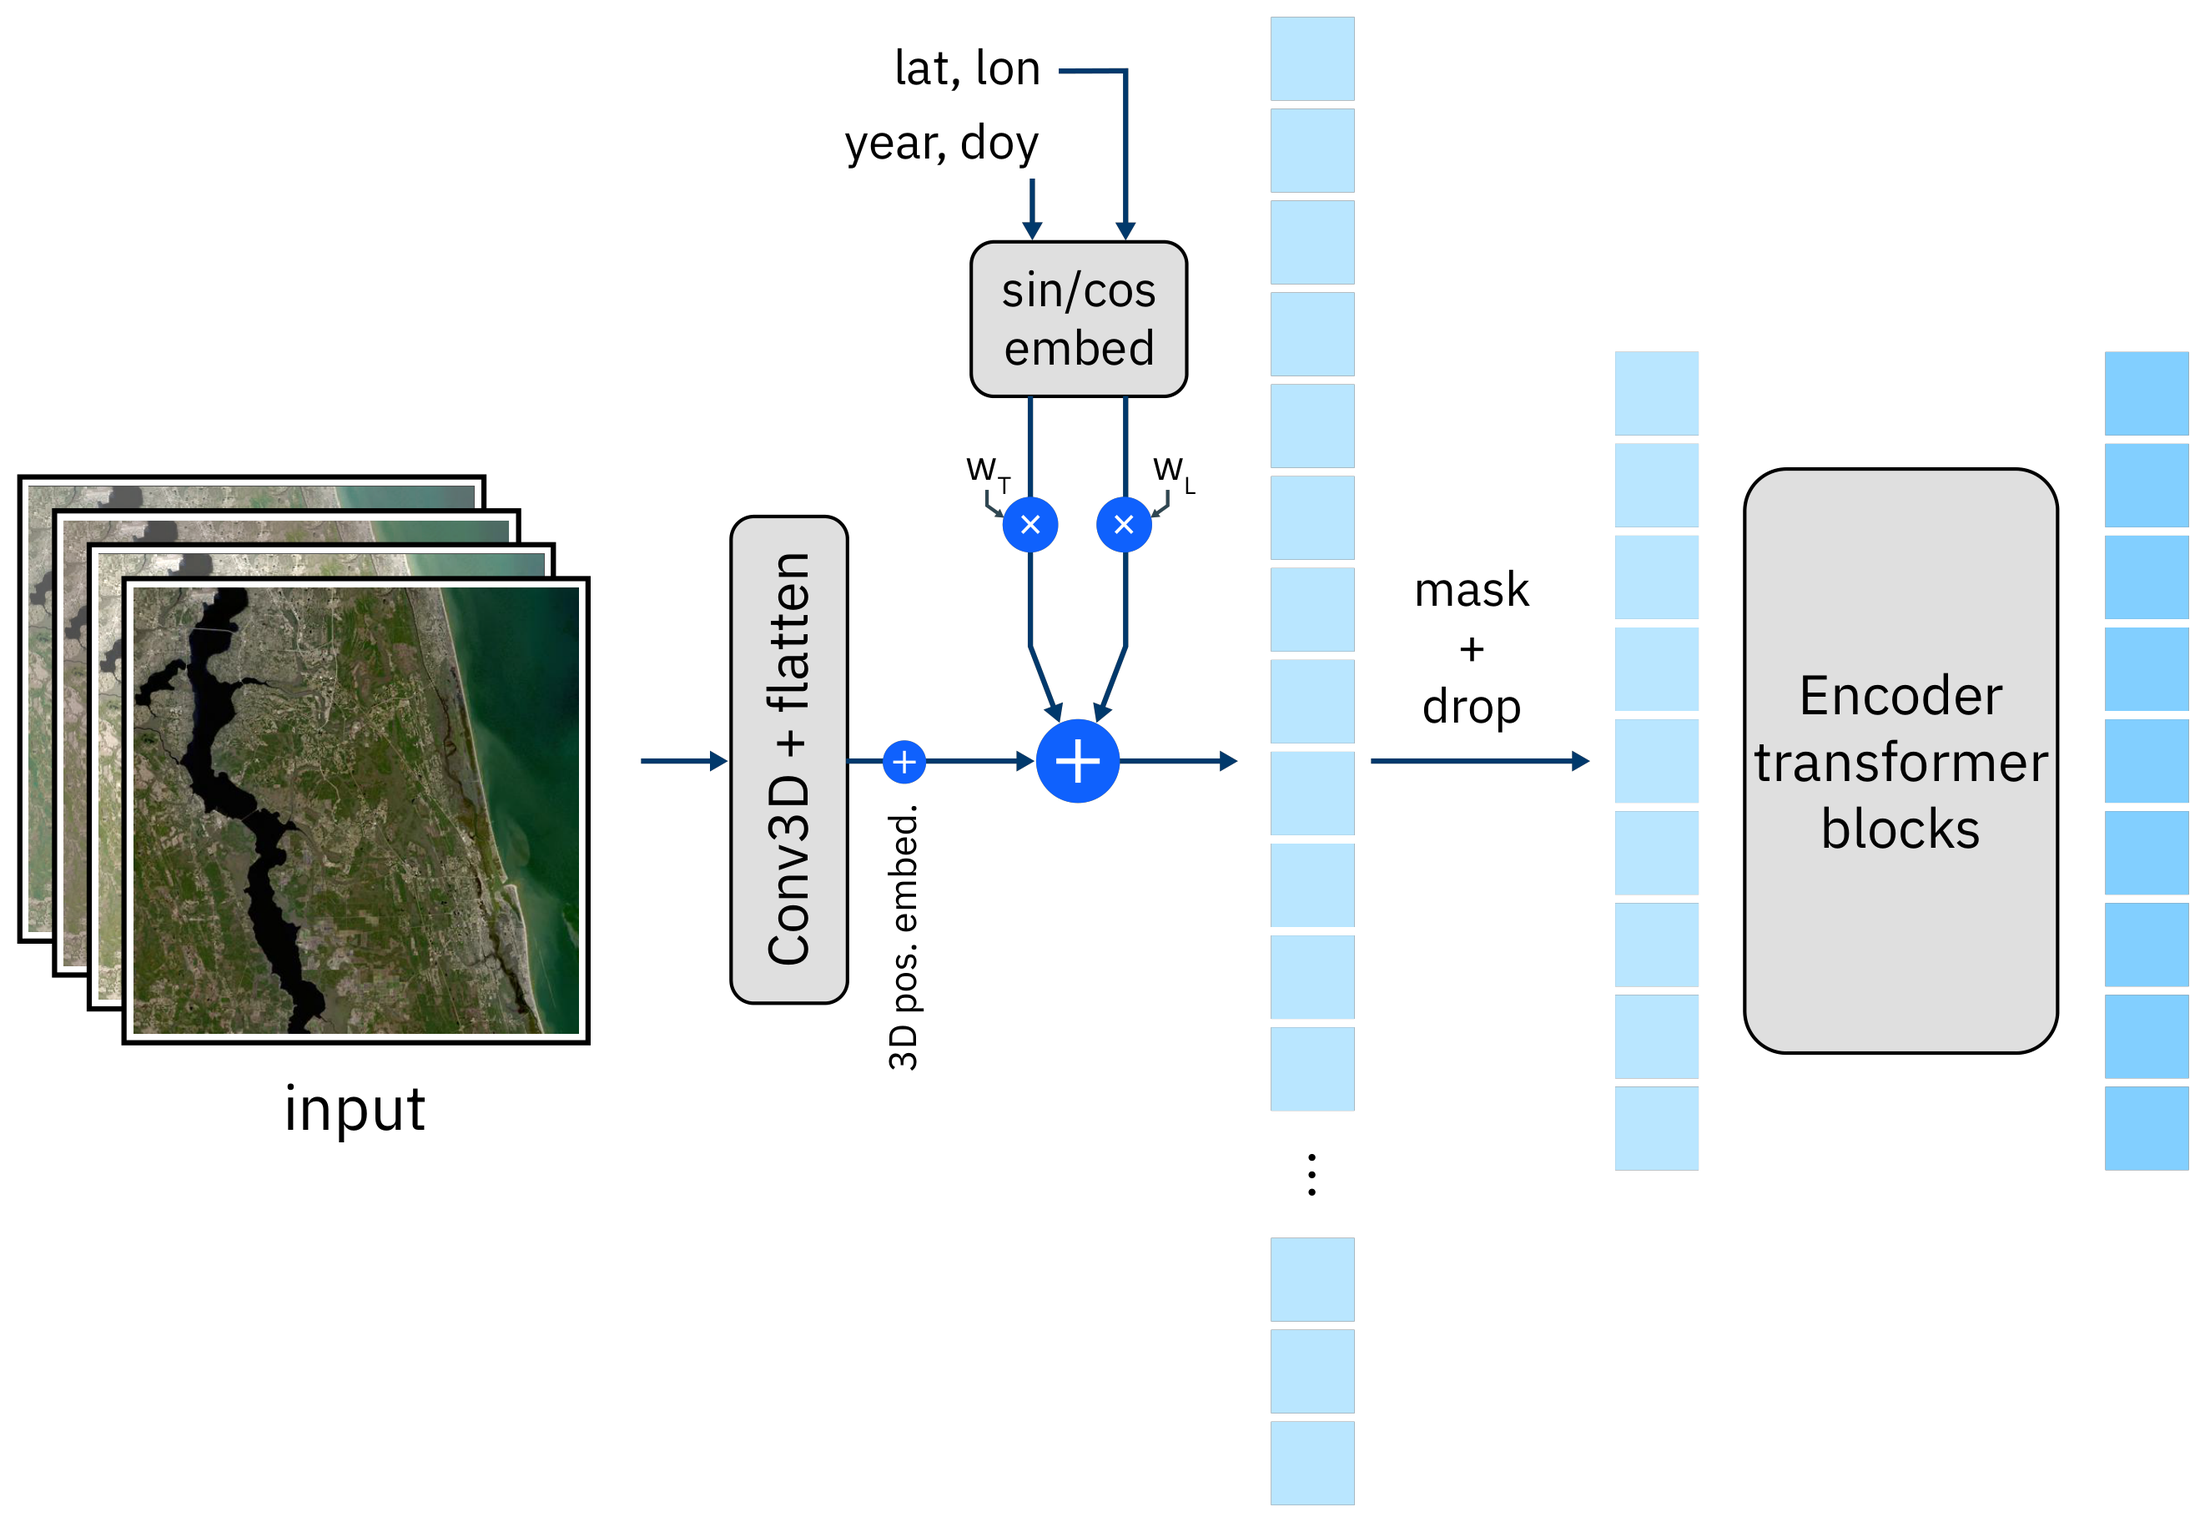
\includegraphics[width=\linewidth,height=0.56\textheight,keepaspectratio]{images/image-restoration-applications/prithvi_eo2_fig3_encoder_metadata.png}\\[0.2em]
      {\scriptsize Date (year, doy = day of year) and location codes, weighted by $w_T$ and $w_L$, are added to every patch token. Szwarcman et al., ``Prithvi-EO-2.0: A Versatile Multi-Temporal Foundation Model for Earth Observation Applications,'' IEEE TGRS 2026, \href{https://arxiv.org/abs/2412.02732v3}{arXiv:2412.02732v3}, Figure~3 (encoder half).\par}
  \end{columns}
\end{frame}

\begin{frame}{AlphaEarth Foundations: An Embedding per Pixel}
  \centering
  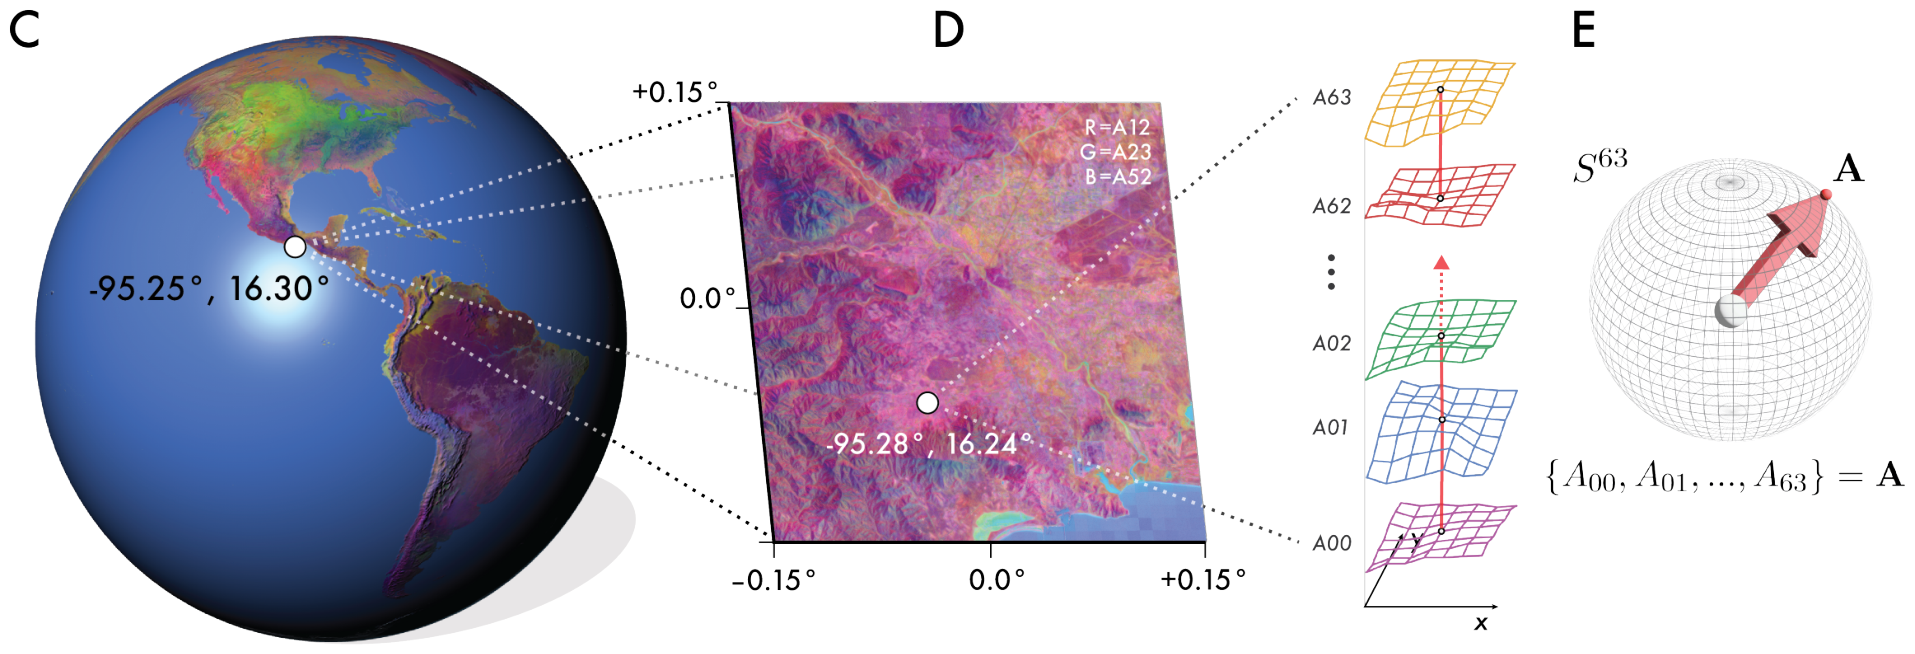
\includegraphics[width=\linewidth,height=0.32\textheight,keepaspectratio]{images/image-restoration-applications/alphaearth_fig1cde_embedding_field.png}\\[0.1em]
  {\scriptsize (C) the 2023 embedding field; (D) three of its 64 axes shown as RGB; (E) every 10\,m pixel is a vector $\mathbf{A}$ on the unit sphere $S^{63}$ in $\mathbb{R}^{64}$. Brown et al., ``AlphaEarth Foundations: An embedding field model for accurate and efficient global mapping from sparse label data,'' arXiv 2025, \href{https://arxiv.org/abs/2507.22291v2}{arXiv:2507.22291v2}, Figure~1(C--E).\par}
  \vspace{0.3em}
  \begin{columns}[T,onlytextwidth]
    \column{0.49\textwidth}
      \begin{itemize}\footnotesize\itemsep0.2em
        \item An \textbf{embedding field} gives every 10\,m pixel a 64-dimensional unit vector summarising its records over a chosen period; the released layers use one year.
        \item Inputs: Sentinel-2, Landsat 8/9 and Sentinel-1. Training also reconstructs PALSAR-2 radar, GEDI LiDAR, elevation, climate and gravity fields, land-cover labels and Wikipedia text as targets, so sparse, irregular records shape one continuous summary.
      \end{itemize}
    \column{0.49\textwidth}
      \begin{itemize}\footnotesize\itemsep0.2em
        \item Mapping becomes a small fit: $k$-NN or a linear layer on the embeddings. Over 15 evaluations with hundreds of labels, error falls by 23.9\% on average against the next-best features (designed: CCDC, MOSAIKS, composites; learned: SatCLIP, Prithvi, Clay); by 10.4\% in ten-shot and 4.18\% in one-shot trials.
        \item The embeddings are released as data, so mapping a region needs labels and a small classifier, with no pretraining.
      \end{itemize}
  \end{columns}
\end{frame}

\begin{frame}{PANGAEA: Foundation Models Against a U-Net}
  \begin{columns}[T,onlytextwidth]
    \column{0.52\textwidth}
      \begin{itemize}\footnotesize\itemsep0.25em
        \item \textbf{Protocol:} 12 open geospatial foundation models, frozen with a trained decoder, against a U-Net and a ViT-B/16 trained from scratch on 11 datasets (floods, burn scars, crops, marine debris, land cover, building damage, biomass), with 100\%, 50\% or 10\% of the labels.
        \item \textbf{Finding:} the foundation models ``do not consistently outperform supervised models''. The U-Net is best on simple low-resolution multispectral tasks: 84.51 mIoU on HLS Burn Scars, 91.42 on Sen1Floods11 (mIoU: IoU averaged over classes).
        \item \textbf{Labels decide:} with 10\% of the labels the U-Net is in the top two on only 2 datasets, and CROMA (contrastive learning plus MAE on paired radar and optical images) on 6.
        \item \textbf{Follow-up:} TerraMind-L reports 59.57 mean mIoU against the U-Net's 57.58, on 9 of the 11 datasets; it left out two whose published scores it could not reproduce.
        \item \textbf{Lesson:} report a supervised U-Net baseline next to any foundation-model result.
      \end{itemize}
    \column{0.46\textwidth}
      \centering
      \vspace{0.4em}
      {\footnotesize Datasets (of 11) on which a model is in the top two\par}
      \vspace{0.3em}
      {\scriptsize
      \begin{tabular}{>{\raggedright\arraybackslash}p{2.6cm} c c c}
        \toprule
        \textbf{Model} & \textbf{100\%} & \textbf{50\%} & \textbf{10\%} \\
        \midrule
        U-Net, from scratch & 6 & 4 & 2 \\
        ViT-B/16, from scratch & 2 & 2 & 3 \\
        \addlinespace[0.2em]
        CROMA & 2 & 4 & 6 \\
        DOFA & 2 & 2 & 2 \\
        Prithvi 1.0 & 1 & 1 & 0 \\
        \bottomrule
      \end{tabular}\par}
      \vspace{0.5em}
      {\scriptsize Marsocci et al., ``PANGAEA: A Global and Inclusive Benchmark for Geospatial Foundation Models,'' arXiv 2024, \href{https://arxiv.org/abs/2412.04204v2}{arXiv:2412.04204v2}, Tables~5--7 (one paragraph of its text gives 5 for the U-Net's full-label count). TerraMind: Jakubik et al., \href{https://arxiv.org/abs/2504.11171v5}{arXiv:2504.11171v5}, Table~6.\par}
  \end{columns}
\end{frame}

\begin{frame}{Vision-Language Models for Earth Observation}
  \begin{columns}[T,onlytextwidth]
    \column{0.52\textwidth}
      \begin{itemize}\footnotesize\itemsep0.25em
        \item \textbf{RemoteCLIP} (TGRS 2024): CLIP retrained for remote sensing. Captioned satellite images are scarce, so detection boxes and segmentation masks are rewritten as captions; with drone images, the training set is 12$\times$ all earlier caption datasets combined. Zero-shot accuracy beats CLIP by up to 6.39\% on average over 12 datasets.
        \item \textbf{GeoChat} (CVPR 2024): LLaVA-1.5 with LoRA on the language model, tuned on 306k remote-sensing instructions generated from labelled datasets. The CLIP encoder runs at 504 instead of 336 pixels for small objects; task tokens (\texttt{[grounding]}, \texttt{[refer]}, \texttt{[identify]}) choose the output, and boxes are text with a rotation angle, coordinates scaled to 0--100.
        \item \textbf{Damage mapping:} xBD pairs pre- and post-disaster images with 850{,}736 building polygons over 45{,}362\,$\mathrm{km}^2$; buildings are outlined in both images, and post-disaster outlines carry a four-level damage label. Comparing two co-registered dates is change detection.
      \end{itemize}
    \column{0.46\textwidth}
      \centering
      \vspace{0.3em}
      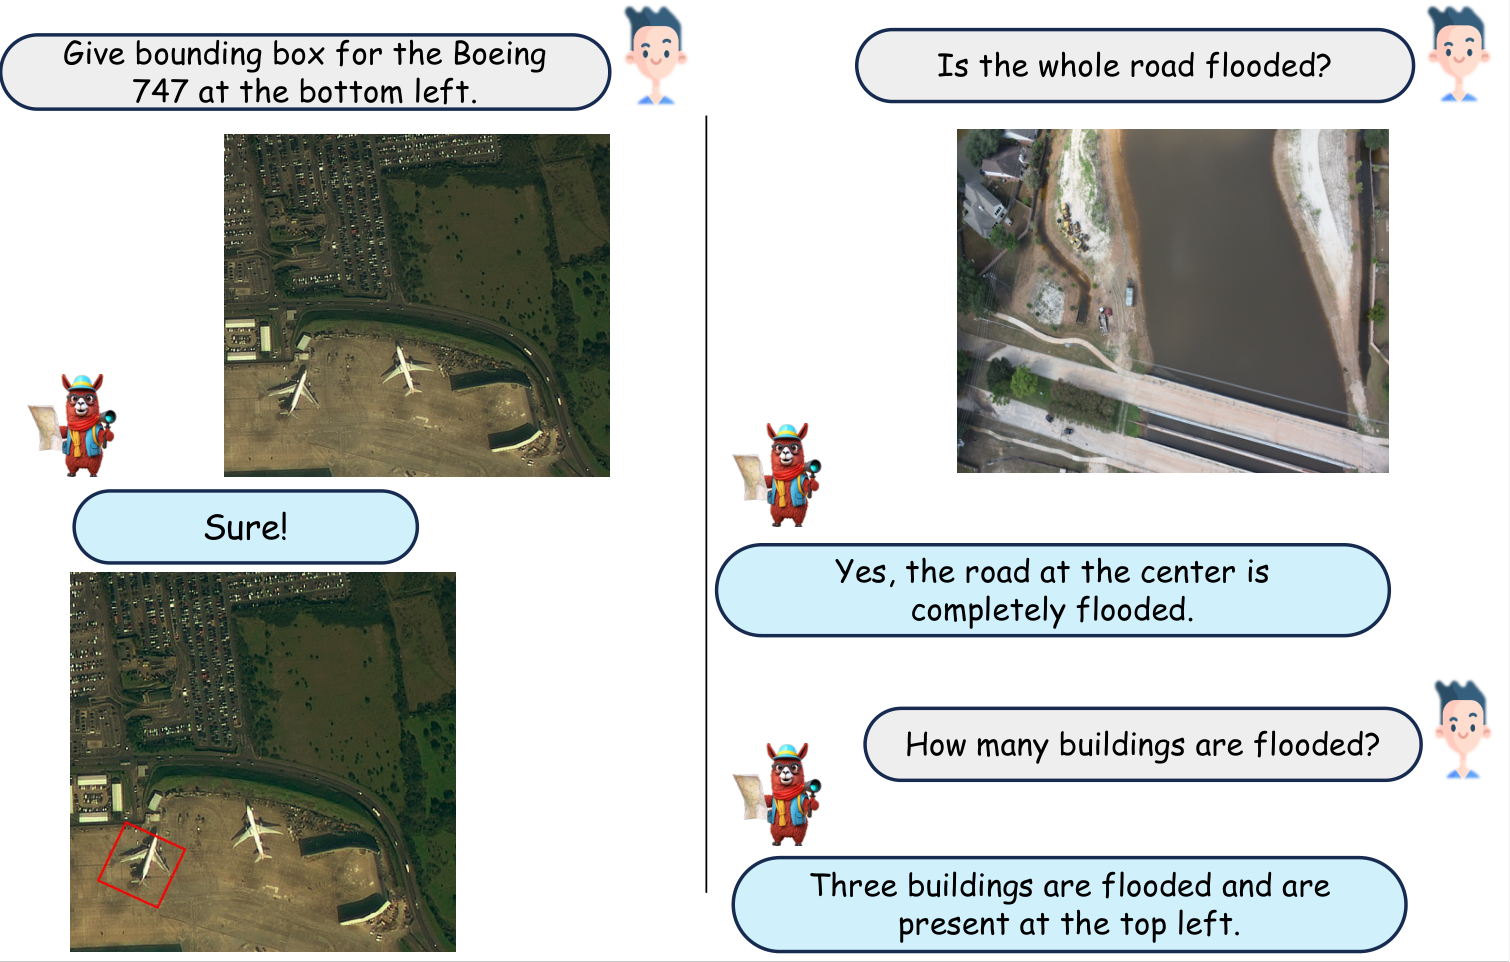
\includegraphics[width=\linewidth,height=0.6\textheight,keepaspectratio]{images/image-restoration-applications/geochat_fig5_grounding_damage_qa.png}\\[0.2em]
      {\scriptsize GeoChat answering with a rotated box (left) and on flood damage (right). Kuckreja et al., ``GeoChat: Grounded Large Vision-Language Model for Remote Sensing,'' CVPR 2024, \href{https://arxiv.org/abs/2311.15826v1}{arXiv:2311.15826v1}, Figure~5 (centre and right panels).\par}
  \end{columns}
\end{frame}

\begin{frame}{Checking Super-Resolved Satellite Images}
  \begin{columns}[T,onlytextwidth]
    \column{0.54\textwidth}
      \begin{itemize}\footnotesize\itemsep0.3em
        \item Generative super-resolution (SR) fills missing detail from its prior. On a satellite image, an invented field edge or track becomes an error in every map built on it.
        \item \textbf{OpenSR-test} (GRSL 2024) scores a result against its low-resolution (LR) input and a real high-resolution (HR) image from another sensor. Each pixel or patch is labelled:
        \begin{itemize}\scriptsize
          \item \textbf{improvement:} detail present in HR and absent in LR;
          \item \textbf{omission:} detail in HR that the result lacks;
          \item \textbf{hallucination:} detail in the result that is not in HR.
        \end{itemize}
        \item It also checks that the result keeps the LR reflectance, spectral signature and position.
        \item Its authors note that PSNR, LPIPS and SSIM ``are not designed to assess SR performance'' when luminance changes or images are misaligned.
      \end{itemize}
    \column{0.44\textwidth}
      \centering
      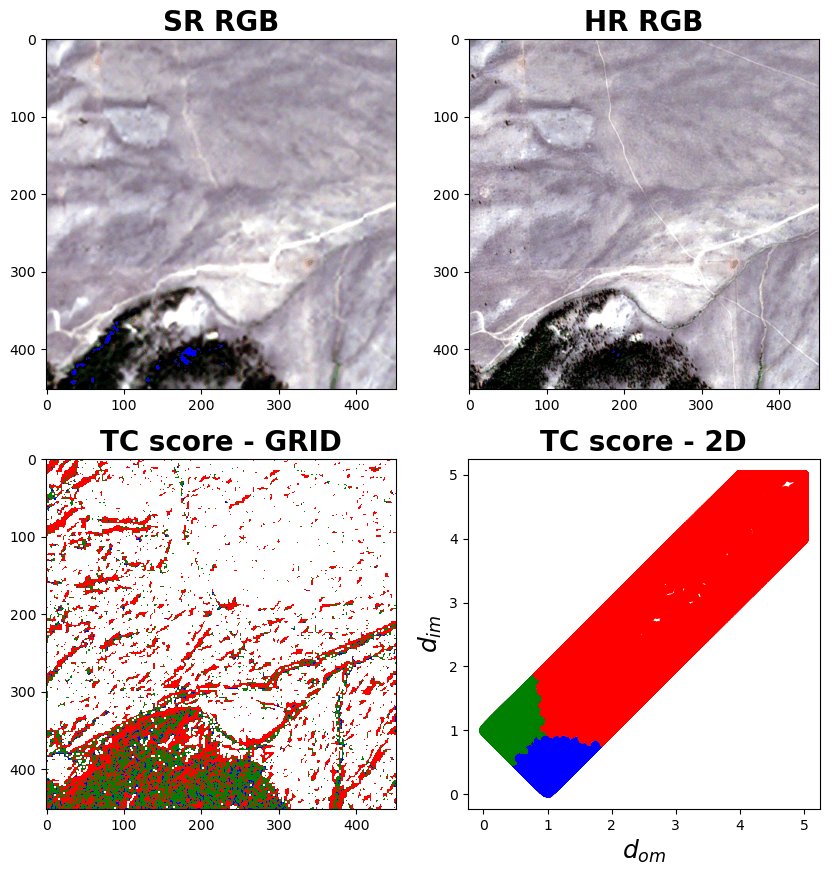
\includegraphics[width=\linewidth,height=0.66\textheight,keepaspectratio]{images/image-restoration-applications/opensr_test_correctness_map.png}\\[0.2em]
      {\scriptsize Red: hallucination; green: omission; blue: improvement. $d_{im}$ and $d_{om}$ are distances to HR and LR in units of the LR--HR distance. Source: \texttt{opensr-test} repository, \href{https://github.com/ESAOpenSR/opensr-test/tree/9e95aeb56a2d6315e8e1c40df6f0aac6dbb09c75}{github.com/ESAOpenSR/opensr-test} (\texttt{docs/images/img\_03.gif}, first frame), MIT licence.\par}
  \end{columns}
\end{frame}

\begin{frame}{Open Earth-Observation Models and Tools}
  All of these are openly released. Sizes are for 16-bit weights: parameters $\times$ 2 bytes.\par
  \vspace{0.6em}
  {\centering\scriptsize
  \begin{tabular}{>{\raggedright\arraybackslash}p{2.5cm} >{\raggedright\arraybackslash}p{5.5cm} >{\raggedright\arraybackslash}p{1.7cm} >{\raggedright\arraybackslash}p{2.6cm}}
    \toprule
    \textbf{Release} & \textbf{What it provides} & \textbf{Licence} & \textbf{Footprint} \\
    \midrule
    TorchGeo & Python library: reprojects rasters to a common coordinate reference system (CRS) and resolution, and samples patches from images too large to load & MIT & library \\
    \addlinespace[0.25em]
    samgeo & runs SAM on GeoTIFF files (images that carry map coordinates) and saves the masks as map polygons & MIT & library \\
    \addlinespace[0.25em]
    Prithvi-EO-2.0 & multi-temporal encoder for Landsat and Sentinel-2 time series & Apache-2.0 & 300M or 600M parameters; 0.6\,GB for 300M \\
    \addlinespace[0.25em]
    TerraMind & any-to-any generative model over nine modalities & Apache-2.0 & tiny, small, base and large released \\
    \addlinespace[0.25em]
    AlphaEarth embeddings & annual 10\,m embedding layers for 2017--2024, as an Earth Engine dataset (bands A00--A63) & CC-BY 4.0 & 64 bytes per pixel at 8 bits \\
    \addlinespace[0.25em]
    GeoChat-7B & remote-sensing vision-language model & Apache-2.0 & about 14\,GB \\
    \bottomrule
  \end{tabular}\par}
  \vspace{0.6em}
  {\scriptsize Sources: \href{https://github.com/torchgeo/torchgeo}{github.com/torchgeo/torchgeo}; \href{https://github.com/opengeos/segment-geospatial}{github.com/opengeos/segment-geospatial}; Hugging Face model cards \href{https://huggingface.co/ibm-nasa-geospatial/Prithvi-EO-2.0-300M}{ibm-nasa-geospatial/Prithvi-EO-2.0-300M}, \href{https://huggingface.co/ibm-esa-geospatial/TerraMind-1.0-base}{ibm-esa-geospatial/TerraMind-1.0-base} and \href{https://huggingface.co/MBZUAI/geochat-7B}{MBZUAI/geochat-7B}; Earth Engine catalog, \href{https://developers.google.com/earth-engine/datasets/catalog/GOOGLE_SATELLITE_EMBEDDING_V1_ANNUAL}{Satellite Embedding V1}.\par}
\end{frame}
